\documentclass[a4paper]{article}

  \usepackage{fullpage} % Package to use full page
  \usepackage{parskip} % Package to tweak paragraph skipping
  \usepackage{tikz} % Package for drawing
  \usepackage{amsmath}
  \usepackage{siunitx}
  \usepackage{amsfonts}
  \usepackage{amssymb}
  \usepackage{hyperref}
  \usepackage[utf8]{inputenc}
  \usepackage[english]{babel}
  \usepackage{multicol}
  \usepackage{graphicx}
  \graphicspath{ {./images/} }
  
  \newcommand\tab[1][0.5cm]{\hspace*{#1}}
  
  \title{Laboratory 7: The Operational Amplifier}
  \author{Adrian Darian}
  \date{11/11/2020}
  
  \begin{document}
  
\maketitle
  
\section*{Objectives}
• Tolearn how to use an operational amplifier (op-amp) constructthree different amplifiercircuits: an inverting amplifier, a non-inverting amplifier, and a difference amplifier. \\
• To learn how the circuit structures and component values affect the output of the circuits. \\
• To learn how to simulate different amplifier circuit with PSPICE. \\

\section*{Equipment and components}
• A desk computer \\
• PSPICE software \\

\section*{Preliminary}
• The op-amp used in this lab is $\si{\mu\ampere}741$, which is one of the cheapest and most popular op-amp. It has open-loop gain and wide operating voltages. The pinout the 741 series is asfollowing. \\
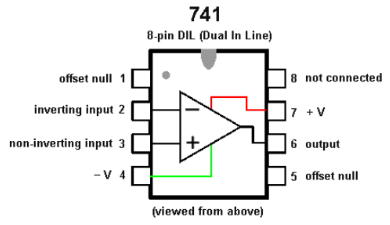
\includegraphics{741.png} \\ 
• Carefully read “Lecture 11” to know what the relationship between the input and output ofeach circuit is and whenthe circuit is operating in the linear operation rangeand fill up thetables in this lab instruction before going to lab. \\
• Review what you have leaned in Lab 8 about howcircuits are simulatedin PSPICE.

\section*{Procedure Version 17.4}
\begin{itemize}
	\item[1.] The Inverting Amplifier
	      \begin{itemize}
	      	\item[1.] A typical inverting amplifier is shown below. \\
	      	      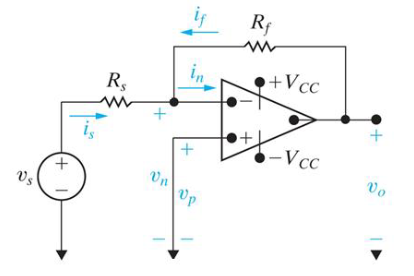
\includegraphics{circuit-1.png} \\ 
	      	      The input is $V_{s}$ and the output is $v_{0}$. If the op amp is ideal, the output voltage is $v_{0} = -\frac{R_{f}}{R_{s}}V_{s}$
	      	\item[2.] Go to the All Program. Under the "PSpice Student", click the "Capture Student" and open the window "OrCAS Capture". Create a new project "Lab 7 inverting".
	      	\item[3.] Click "Place|parts...", add all libraries. Then place "$\si{\mu\ampere}741$", and resistors "$R_{f}$" and "$R_{s}$", "Vdc"and set Vdc = 12V. Place "$V_{sin}$" and set Voff = 0, Vampl = 2V, Freq = 100Hz. Place a couple of "ground 0". Set $R_{s}$ = $\SI{1}{\kilo\ohm}$.
	      	\item[4.] Use "wire" to connect all parts. Set voltage measurement points as shown below.
	      	\item[5.] Click "New SImulation". Set a name "Lab 7 inverting".
	      	\item[6.] Click "Simulation Settings" Under "Analysis Type", select "Time Domain". Under "Options", check "General Settings". Fill in the "Run to time" box with 50ms, "Start saving data after" with 0, and "Maximum step size" with $\SI{5}{\mu}s$.
	      	\item[7.] Fill up the peak vale of each voltage for the different values of $R_{f}$. \\
	      	      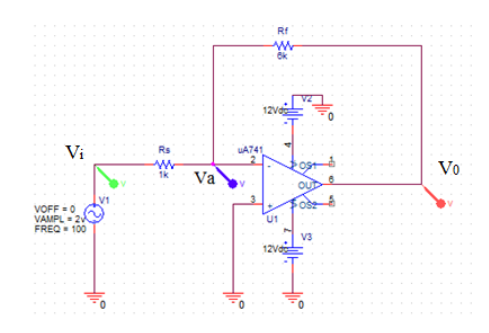
\includegraphics{circuit-2.png} \\      
	      \end{itemize}
	      \begin{tabular}{|l|l|l|l|l|l|l|l|}
	      	\hline
	      	$R_{f}(\si{\kilo\ohm})$ & 0.1  & 0.5   & 1     & 4     & 6       & 8       & 10      \\
	      	\hline
	      	$V_{im}(V) (VAMPL)$     & 2    & 2     & 2     & 2     & 2       & 2       & 2       \\
	      	\hline
	      	$V_{am}(V)$             & 0    & 0     & 0     & 0     & 0       & 0       & 0       \\
	      	\hline
	      	$V_{om}(V)$             & 200  & -0.99 & -1.99 & -7.99 & -11.602 & -11.613 & -11.613 \\
	      	\hline
	      	$G(Closed-gain)$        & -100 & 0.495 & 0.995 & 3.995 & 5.801   & 5.8065  & 5.8065  \\
	      	\hline
	      \end{tabular} \\
	      What do you observer? Explain them by using what you learned in class. Calculate the currents $i_{s}$ and $i_{f}$ based on the voltages in the table above and fill up the table below. \\
	      \begin{tabular}{|l|l|l|l|l|l|l|l|}
	      	\hline
	      	$R_{f}(\si{\kilo\ohm})$     & 0.1      & 0.5     & 1      & 4      & 6      & 8     & 10      \\
	      	\hline
	      	$i_{s}(\si{\milli\ampere})$ & 2        & 2       & 2      & 2      & 2      & 2     & 2       \\
	      	\hline
	      	$i_{f}(\si{\milli\ampere})$ & -1.99968 & -1.9998 & -1.999 & -1.998 & -1.934 & -1.45 & -1.1613 \\
	      	\hline
	      \end{tabular} \\
	      What do you find from the data in the table above?
	\item[2.] The Noninverting Amplifier
	      \begin{itemize}
	      	\item[1.] A typical noninverting amplifier circuit is shown below. \\
	      	      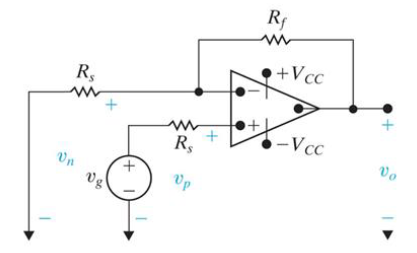
\includegraphics{circuit-3.png} \\
	      	      The input is $v_{s}$ and the output is $v_{0}$. If the op amp is ideal, the output voltage is $v_{o} = (1 + \frac{R_{f}}{R_{s}})V_{s}$.
	      	\item[2.] Creat a new project "Lab 7 noninverting". CLick "Place|parts...", add all libraries. Then place "$\si{\mu\ampere}741$", right click on the "$\si{\mu\ampere}741$" and then click "Mirror Vertically". Place resistors "$R_{f}$" and "$R_{s}$", "Vdc" and set Vdc = 12V. Place "$V_{sin}$" and set Voff = 0, Vampl = 2V, Freq = 100Hz. Place a couple of "ground 0". Set $R_{s1} = R_{s2} = \SI{1}{\kilo\ohm}$.
	      	\item[3.] Use "wire" to connect all parts. Set voltage measurement points as shown below.
	      	\item[4.] Click "New Simulation". Set a name "Lab 7 noninverting".
	      	\item[5.] Click "Simulation Settings". Under "Analysis Type", select "Time Domain". Under "Options", check "General Settings". Fill in the "Run to time" box with 50ms, "Start saving data after" with 0, and "maximum step size" with $\SI{5}{\mu}s$.
	      	\item[6.] Fill up the peak value of each voltage for the different values of $R_{f}$.  
	      \end{itemize} 
	      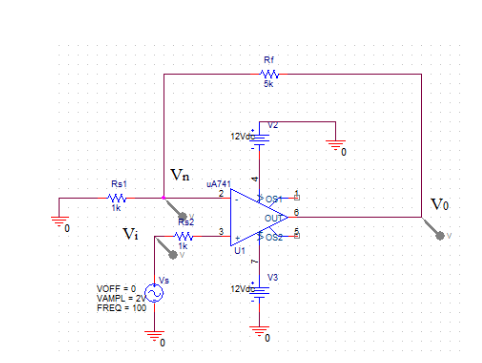
\includegraphics{circuit-4.png} \\
	      \begin{tabular}{|l|l|l|l|l|l|l|}
	      	\hline
	      	$R_{f}(\si{\kilo\ohm})$ & 0.1    & 0.5  & 1    & 4    & 8      & 10     \\
	      	\hline
	      	$V_{im}(V)$             & 2      & 2    & 2    & 2    & 2      & 2      \\
	      	\hline
	      	$V_{om}(V)$             & 2.19   & 3    & 4    & 10   & 11.61  & 11.61  \\
	      	\hline
	      	$V_{nm}(V)$             & 1.99   & 1.99 & 1.99 & 1.99 & 1.29   & 1.056  \\
	      	\hline
	      	$G(Closed-gain)$        & -1.095 & -1.5 & -2   & -5   & -5.805 & -5.805 \\
	      	\hline
	      \end{tabular} \\
	      What do you observe? Explain them by using what you learned in class.
	\item[3.] The Difference Amplifier
	      \begin{itemize}
	      	\item[1.] A typical noninverting amplifier circuit is shown below. \\
	      	      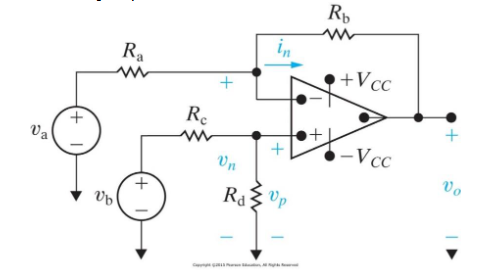
\includegraphics{circuit-5.png} \\
	      	      The inputs are $v_{a}$ and $v_{b}$, the output is $v_{0}$. If the op amp is ideal, the output voltage is $v_{0} = \frac{R_{d}(R_{a} + R_{b})}{R_{a}(R_{c} + R_{d})}V_{b} - \frac{R_{b}}{R_{a}}v_{a}$. \\
	      	      If $\frac{R_{a}}{R_{b}} = \frac{R_{c}}{R_{d}}, v_{0} = \frac{R_{b}}{R_{a}}(v_{b} - v_{a})$, which means the output voltage is proportional to the difference of the two inputs.
	      	\item[2.] Create a new project "Lab 7 difference". Click "Place|parts...", add all libraries. Then place "$\si{\mu\ampere}741$", right click on then "$\si{\mu\ampere}741$" and then click  "Mirror Vertically". Place and set resistors "$R_{a} = \SI{1}{\kilo\ohm}$", "$R_{b} = \SI{1}{\kilo\ohm}$", "$R_{c} = \SI{1}{\kilo\ohm}$", and "$R_{d} = \SI{1}{\kilo\ohm}$". Place "Vdc" and set Vdc = 12V. Place "$V_{sin}$" and set Voff = 0, Vample = 2V, Freq = 100Hz. Place a couple of "ground 0".
	      	\item[3.] Use "wire" to connect all parts. Set voltage measurement points as shown below.
	      	\item[4.] Click "New Simulation". Set a name "Lab 7 difference".
	      	\item[5.] Click "Simulation Settings". Fill in the "Run to time" box with 50ms, "Start saving data after" with 0, and "Maximum step size" with $\SI{5}{\mu}s$.
	      	\item[6.] Fill up the peak value of each voltage for the different values of $V_{bm}$.   
	      \end{itemize} 
	      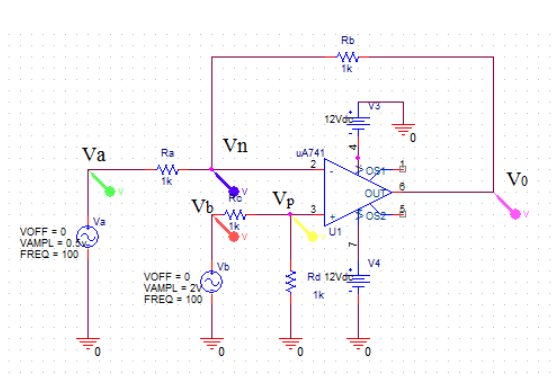
\includegraphics{circuit-6.png} \\
	      \begin{tabular}{|l|l|l|l|l|l|l|}
	      	\hline
	      	$V_{am}(V)$      & 0.5    & 0.5    & 0.5   & 0.5   & 0.5     & 0.5    \\
	      	\hline
	      	$V_{bm}(V)$      & -0.5   & 0      & 0.5   & 1     & 5       & 15     \\
	      	\hline
	      	$V_{nm}(V)$      & -0.250 & 0      & 0.249 & 0.499 & 2.5     & 6.057  \\
	      	\hline
	      	$V_{pm}(V)$      & -0.250 & 0      & 0.249 & 0.499 & 2.5     & 7.499  \\
	      	\hline
	      	$V_{om}(V)$      & -0.999 & -0.499 & 0     & 0.5   & 4.499   & 11.614 \\
	      	\hline
	      	$G(Closed-gain)$ & 1.0    & 0.9998 & 1     & 1     & 0.99997 & 1.0001 \\
	      	\hline
	      \end{tabular}
\end{itemize}

\section*{Questions and Conclusions}
What do you find from the simulation results? \\
• Summarize your findings ofthis lab. \\
\tab Through this lab we saw how an op amp behaved in different situations. In the inverting amplifier circuit the $V_{im}$ and $V_{am}$ remained constant as $R_{f}$ was increased and  $V_{om}$ and $G$ increased in magnitude. We noticed in the inverting amplifier circuit that the $G$ closed gain valued hovered around $5.8$ as we increased the value of $R_{f}$. This same pattern is also noticeable in the non-inverting amplifier. In the difference amplifier, the $V_{nm}$ and $V_{pm}$ produced similar values but, $V_{om}$ had very different results other than when $V_{bm} = 0.5$. The $G$ closed gain consistently stayed around $1.0$ despite changing the $V_{bm}$ values. Overall these calculations and data show how the different op amps behave and how we can calculate the values of using the op amp equations. 

\end{document}